\section{Theory}

\sectioncover

\subsection{Thermodynamics}

\begin{frame}
  \vspace{-2em}
  \begin{columns}
    \begin{column}{0.4\textwidth}
      \begin{itemize}
        \item  Working with the Helmholtz free energy density $\psi$, variables we are concerned with are
              \begin{align*}
                \bs{\upphi}, \quad \defgrad^p, \quad \ep, \quad d, \quad T.
              \end{align*}
        \item Conservations and thermodynamic laws:
              \begin{align*}
                 & \dot{\rho_0} = 0,                                                                             \\
                 & \rho_0 \bta = \divergence \bfP + \rho_0\btb,                                                  \\
                 & \bfP\defgrad = \defgrad\bfP^T,                                                                \\
                 & f -\divergence \bs{\xi} = 0,                                                                  \\
                 & \dot{u} + \dot{k} = \mathcal{P}^\text{ext} + \rho_0 q - \divergence \bth,                     \\
                 & \dot{s}^\text{int} = \dot{s} - \dfrac{\rho_0 q}{T} + \divergence \dfrac{\bth}{T} \geqslant 0. 
              \end{align*}
      \end{itemize}
    \end{column}
    \pause
    \begin{column}{0.6\textwidth}
      \begin{itemize}
        \item Generalized forces are
              \begin{align*}
                 & \bfP = \bfP^\text{eq} + \bfP^\text{vis}, \quad \bfT = \bfT^\text{eq} + \bfT^\text{vis}, \quad Y = Y^\text{eq} + Y^\text{vis}, \\
                 & f = f^\text{eq} + f^\text{vis}, \quad \bs{\xi} = \bs{\xi}^\text{eq} + \bs{\xi}^\text{vis},                                    
              \end{align*}
        \item Following the Coleman-Noll procedure:
              \begin{align*}
                 & \bfP^\text{eq} = \psi_{,\defgrad}, \quad \bfT^\text{eq} = \psi_{,\defgrad^p}, \quad Y^\text{eq} = \psi_{,\ep}, \\
                 & f^\text{eq} = \psi_{,d}, \quad \bs{\xi}^\text{eq} = \psi_{,\grad d}, \quad -s = \psi_{,T}.                     
              \end{align*}
        \item Viscous forces follow from the dual kinetic potential $\Delta^*$:
              \begin{align*}
                 & \bfP^\text{vis} = \Delta^*_{,\dot{\defgrad}}, \quad \bfT^\text{vis} = \Delta^*_{,\dot{\defgrad}^p}, \quad Y^\text{vis} = \Delta^*_{,\epdot}, \\
                 & f^\text{vis} = \Delta^*_{,\dot{d}}, \quad \bs{\xi}^\text{vis} = \Delta^*_{,\grad\dot{d}}.                                                    
              \end{align*}
        \item To satisfy the second law:
              \begin{align*}
                \delta = \bfP^\text{vis}:\dot{\defgrad} + \bfT^\text{vis}:\dot{\defgrad}^p + Y^\text{vis}\epdot + f^\text{vis}\dot{d} + \bs{\xi}^\text{vis}\cdot\grad \dot{d} \geqslant 0.
              \end{align*}
      \end{itemize}
    \end{column}
  \end{columns}
\end{frame}

\subsection{The variational statement}

\begin{frame}
  With $\mathcal{V} = \{ \defrate, \dot{\defgrad}^p, \epdot, \dot{d} \}$:
  \begin{block}{}
    \vspace{-0.5em}
    \begin{align*}
      \left( \mathcal{V}, \dot{s}, T \right) & = \arg \left( \inf_{\mathcal{V}, \dot{s}} \sup_T L \right),        \\
      L                                      & = \int\limits_{\body_0} \varphi \diff{V} - \mathcal{P}^\text{ext}, \\
      \varphi                                & = \dot{k} + \dot{u} + \Delta^* - T\dot{s} - \chi,                  
    \end{align*}
  \end{block}
\end{frame}

\subsection{Constitutive choices}

\begin{frame}
  \vspace{-1.5em}
  \begin{block}{}
    \begin{align*}
      L = \int\limits_{\body_0} \left[ \textcolor<1>{red}{\dot{\psi}^e} + \textcolor<2>{red}{{\psi^e}^*} + \textcolor<4>{red}{\dot{\psi}^p} + \textcolor<4>{red}{{\psi^p}^*} + \textcolor<5>{red}{\dot{\psi}^f} + \textcolor<5>{red}{{\psi^f}^*} - T\dot{s} - \textcolor<6>{red}{\chi} \right] \diff{V} - \textcolor<7>{red}{\mathcal{P}^\text{ext}}, \\
      \textcolor<3,5>{red}{\text{subject to } \bfL(\bfZ) \dot{\bfZ} = \bs{0}}.
    \end{align*}
  \end{block}
  
  \begin{overlayarea}{\textwidth}{0.4\textwidth}
    \only<1>{
      \begin{columns}[T]
        \begin{column}{0.5\textwidth}
          Option 1 (Compressible Neo-Hookean):
          \begin{align*}
            \psi^e               = & \ g \psi^e_\activepart + \psi^e_\inactivepart,                                                                \\
            \psi^e_\activepart   = & \ \mathbb{H}_1(J)\left\{ \dfrac{1}{2}K\left[ \dfrac{1}{2}(J^2-1) - \ln(J) \right] \right\}                    \\
                                   & \ + \dfrac{1}{2}G\left( \overbar{\bfC}:{\bfC^p}^{-1} - 3 \right),                                             \\
            \psi^e_\inactivepart = & \ \left( 1-\mathbb{H}_1(J) \right) \left\{ \dfrac{1}{2}K\left[ \dfrac{1}{2}(J^2-1) - \ln(J) \right] \right\}. 
          \end{align*}
        \end{column}
        \begin{column}{0.5\textwidth}
          Option 2 (Hencky):
          \begin{align*}
            \psi^e               & =  g \psi^e_\activepart + \psi^e_\inactivepart,                                       \\
            \psi^e_\activepart   & = \dfrac{1}{2} K \macaulay{\tr(\strain^e)}_+^2 + G \dev{\strain^e} : \dev{\strain^e}, \\
            \psi^e_\inactivepart & = \dfrac{1}{2} K \macaulay{\tr(\strain^e)}_-^2,                                       \\
            \strain^e            & = \frac{1}{2} \ln\left( \bfC^e \right).                                               
          \end{align*}
        \end{column}
      \end{columns}
    }
    
    \only<2>{
      \begin{columns}
        \begin{column}{0.5\textwidth}
          Newtonian viscosity:
          \begin{align*}
            {\psi^e}^* & = g J \left[ \dfrac{1}{2}\zeta \tr(\bfd)^2 + \eta \bfd:\bfd \right], \\
            \bfd       & = \sym\left( \dot{\defgrad}\defgrad^{-1} \right).                    
          \end{align*}
        \end{column}
      \end{columns}
    }
    
    \only<3>{
      \begin{columns}[T]
        \begin{column}{0.4\textwidth}
          Flow rule constraints:
          \begin{align*}
            \tr\left( \dot{\defgrad}^p{\defgrad^p}^{-1} \right) = 0, \\
            \norm{\dot{\defgrad}^p{\defgrad^p}^{-1}}^2 - \frac{3}{2} \abs{\epdot}^2 = 0.
          \end{align*}
        \end{column}
        \begin{column}{0.6\textwidth}
          \vspace{-0.5em}
          \begin{remark}[Flow rule]
            The joint minimization problem
            \begin{align*}
              \left( \dot{\defgrad}^p, \epdot \right) = & \ \arg\inf_{\dot{\defgrad}^p, \epdot} \left[ \bfT^\text{eq}:\dot{\defgrad}^p + Y^\text{eq}\epdot + \Delta^* \right] 
            \end{align*}
            recovers the Prandtl-Reuss flow rule:
            \begin{align*}
              \dot{\defgrad}^p{\defgrad^p}^{-1} = \epdot \bfN^p, \quad \bfN^p = \sqrt{\dfrac{3}{2}}\dfrac{\dev(\bfM)}{\norm{\dev(\bfM)}},
            \end{align*}
            and the loading/unloading conditions:
            \begin{align*}
               & \phi^p \leqslant 0, \quad \epdot \geqslant 0, \quad \phi^p\epdot = 0,                       \\
               & \phi^p = \norm{\dev(\bfM)} - \sqrt{\dfrac{2}{3}} \left( Y^\text{eq} + Y^\text{vis} \right). 
            \end{align*}
          \end{remark}
        \end{column}
      \end{columns}
    }
    
    \only<4>{
      \textcolor{red}{
        \begin{align*}
          \psi^p     & = ? \\
          {\psi^p}^* & = ? 
        \end{align*}
      }
    }
    
    \only<5>{
      \begin{columns}[T]
        \begin{column}{0.5\textwidth}
          Fracture energy density:
          \begin{align*}
            \psi^f = \dfrac{\Gc}{c_0l}\left( \alpha + l^2 \grad d \cdot \grad d \right).
          \end{align*}
          Viscous regularization:
          \textcolor{red}{
            \begin{align*}
              {\psi^f}^* = ?.
            \end{align*}
          }
          Irreversibility constraint:
          \begin{align*}
            \dot{d} \geqslant 0.
          \end{align*}
        \end{column}
        \begin{column}{0.5\textwidth}
          \begin{remark}[Propagation envelope]
            The fracture propagation envelope follows as:
            \begin{align*}
              \phi^f & =\divergence \dfrac{2\Gc l}{c_0} \grad d - \left( \dfrac{\Gc}{c_0 l}\alpha_{,d} + \psi^d + f^\text{vis} \right), \\
              \psi^d & = \psi^e_{,d} + \psi^p_{,d}.                                                                                     
            \end{align*}
          \end{remark}
          \textcolor{red}{
            \begin{align*}
              \alpha & = ? \\
              g      & = ? 
            \end{align*}
          }
        \end{column}
      \end{columns}
    }
    
    \only<6>{
      Fourier potential describes heat conduction:
      \begin{align*}
        \chi & = \dfrac{1}{2}\kappa\btg\cdot\btg, \\
        \btg & = - \grad T / T.                   
      \end{align*}
    }
    
    \only<7>{
      The external power expenditure $\mathcal{P}^\text{ext}$ is defined as
      \begin{equation*}
        \begin{aligned}
          \mathcal{P}^\text{ext} = & \ \underbrace{\int\limits_{\body_0} \rho_0 \btb \cdot \defrate \diff{V}}_\text{body force} + \underbrace{\int\limits_{\partial_t\body_0} \btt \cdot \defrate \diff{A}}_\text{surface traction} + \underbrace{\int\limits_{\partial_h\body_0} \bar{h}_n\ln\left( \dfrac{T}{T_0} \right) \diff{A}}_\text{external heat flux} \\
                                   & + \underbrace{\int\limits_{\partial_r\body_0} h\left[ T - T_0 \ln\left( \dfrac{T}{T_0} \right) \right] \diff{A}}_\text{external heat convection} - \underbrace{\int\limits_{\body_0} \rho_0 q \ln\left( \dfrac{T}{T_0} \right) \diff{V}}_\text{heat source},                                                               
        \end{aligned}
      \end{equation*}
    }
  \end{overlayarea}
\end{frame}

\subsection{Model construction}

\begin{frame}
  \small
  \vspace{-2em}
  \begin{block}{Plasticity and fracture envelopes}
    \vspace{-1em}
    \begin{align*}
      \phi^p & = \norm{\dev(\bfM)} - \sqrt{\dfrac{2}{3}} \left( \psi^p_{,\ep} + {\psi^p}^*_{,\epdot} \right) \leqslant 0,                                                \\
      \phi^f & = \divergence \dfrac{2\Gc l}{c_0} \grad d - \left( \dfrac{\Gc}{c_0 l}\alpha_{,d} + \psi^e_{,d} + \psi^p_{,d} + {\psi^f}^*_{,\dot{d}} \right) \leqslant 0. 
    \end{align*}
  \end{block}
  
  \begin{overlayarea}{\textwidth}{0.4\textwidth}
    \only<1>{
      \begin{columns}
        \begin{column}{0.4\textwidth}
          \textboxed{Version 0} \\\bigskip
          
          Constitutive choices:
          \begin{align*}
            \psi^p     & = \sigma_y \ep + \dfrac{1}{2} H \ep^2, \\
            {\psi^p}^* & = 0,                                   \\
            {\psi^f}^* & = \dfrac{1}{2} v \dot{d}^2,            \\
            \alpha     & = d^2,                                 \\
            g          & = (1-d)^2.                             
          \end{align*}
        \end{column}
        \begin{column}{0.6\textwidth}
          Resulting envelopes:
          \begin{align*}
            \norm{\dev(\bfM)} - \sqrt{\dfrac{2}{3}} \psi^p_{,\ep}                                                & \leqslant 0,         \\
            \divergence \dfrac{2\Gc l}{c_0} \grad d - \left( \dfrac{\Gc}{c_0 l}\alpha_{,d} + \psi^e_{,d} \right) & \leqslant v \dot{d}. 
          \end{align*}
          Issue: Crack propagates along the plastic zone in reality.
          \begin{figure}
            \centering
            \begin{subfigure}{0.4\textwidth}
              \centering
              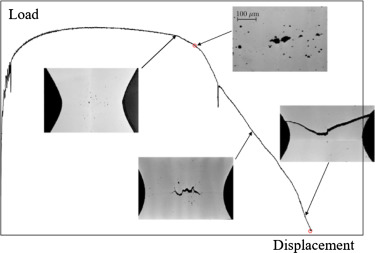
\includegraphics[width=1\textwidth]{theory/figures/coupling}
            \end{subfigure}
            \begin{subfigure}{0.4\textwidth}
              \centering
              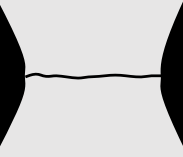
\includegraphics[width=0.5\textwidth]{theory/figures/no_coupling}
            \end{subfigure}
          \end{figure}
        \end{column}
      \end{columns}
    }
    
    \only<2>{
      \begin{columns}
        \begin{column}{0.4\textwidth}
          \textboxed{Version 1} \\\bigskip
          
          Constitutive choices:
          \begin{align*}
            \psi^p     & = \textcolor{red}{g} \left( \sigma_y \ep + \dfrac{1}{2} H \ep^2 \right), \\
            {\psi^p}^* & = 0,                                                                     \\
            {\psi^f}^* & = \dfrac{1}{2} v \dot{d}^2,                                              \\
            \alpha     & = d^2,                                                                   \\
            g          & = (1-d)^2.                                                               
          \end{align*}
        \end{column}
        \begin{column}{0.6\textwidth}
          Resulting envelopes:
          \begin{align*}
            \norm{\dev(\bfM)} - \sqrt{\dfrac{2}{3}} \textcolor{red}{\psi^p_{,\ep}}                                                              & \leqslant 0,         \\
            \divergence \dfrac{2\Gc l}{c_0} \grad d - \left( \dfrac{\Gc}{c_0 l}\alpha_{,d} + \psi^e_{,d} + \textcolor{red}{\psi^p_{,d}} \right) & \leqslant v \dot{d}. 
          \end{align*}
          \begin{columns}
            \begin{column}[t]{0.5\textwidth}
              Improvement: Fracture and plasticity are now strongly coupled.
              \begin{figure}
                \centering
                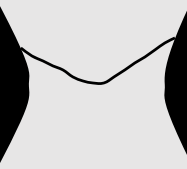
\includegraphics[width=0.45\textwidth]{theory/figures/strong_coupling}
              \end{figure}
            \end{column}
            \begin{column}[t]{0.5\textwidth}
              Issue: The response is altered by the onset of damage.
              \begin{figure}
                \centering
                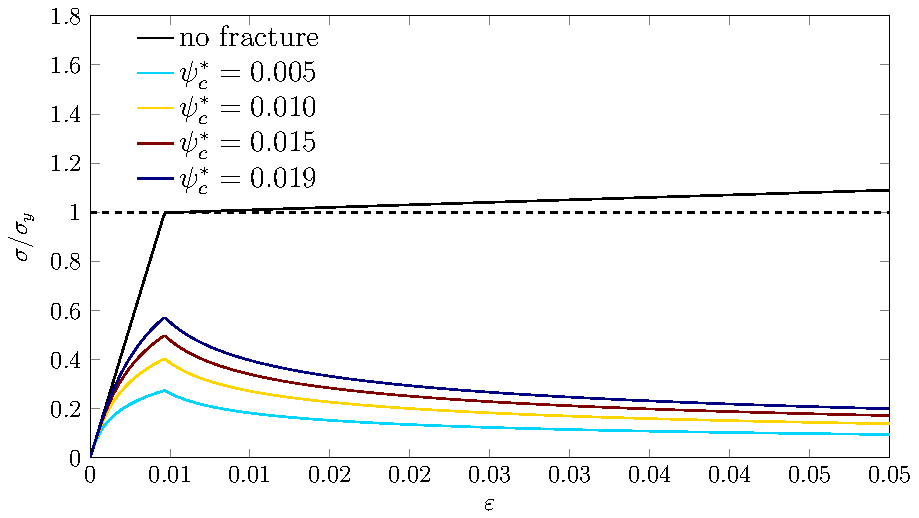
\includegraphics[width=0.9\textwidth]{theory/figures/Chapter5-homogenized-compare_alpha-EPPD_xi_0}
              \end{figure}
            \end{column}
          \end{columns}
        \end{column}
      \end{columns}
    }
    
    \only<3>{
      \begin{columns}
        \begin{column}{0.4\textwidth}
          \textboxed{Version 2} \\\bigskip
          
          Constitutive choices:
          \begin{align*}
            \psi^p     & = g \left( \sigma_y \ep + \dfrac{1}{2} H \ep^2 \right), \\
            {\psi^p}^* & = 0,                                                    \\
            {\psi^f}^* & = \dfrac{1}{2} v \dot{d}^2,                             \\
            \alpha     & = \textcolor{red}{d},                                   \\
            g          & = (1-d)^2.                                              
          \end{align*}
        \end{column}
        \begin{column}{0.6\textwidth}
          Resulting envelopes:
          \begin{align*}
            \norm{\dev(\bfM)} - \sqrt{\dfrac{2}{3}} \psi^p_{,\ep}                                                                                & \leqslant 0,         \\
            \divergence \dfrac{2\Gc l}{c_0} \grad d - \left( \dfrac{\Gc}{c_0 l} \textcolor{red}{\alpha_{,d}} + \psi^e_{,d} + \psi^p_{,d} \right) & \leqslant v \dot{d}. 
          \end{align*}
          \begin{columns}
            \begin{column}[t]{0.5\textwidth}
              Improvement: A purely elastoplastic stage.
              \begin{figure}
                \centering
                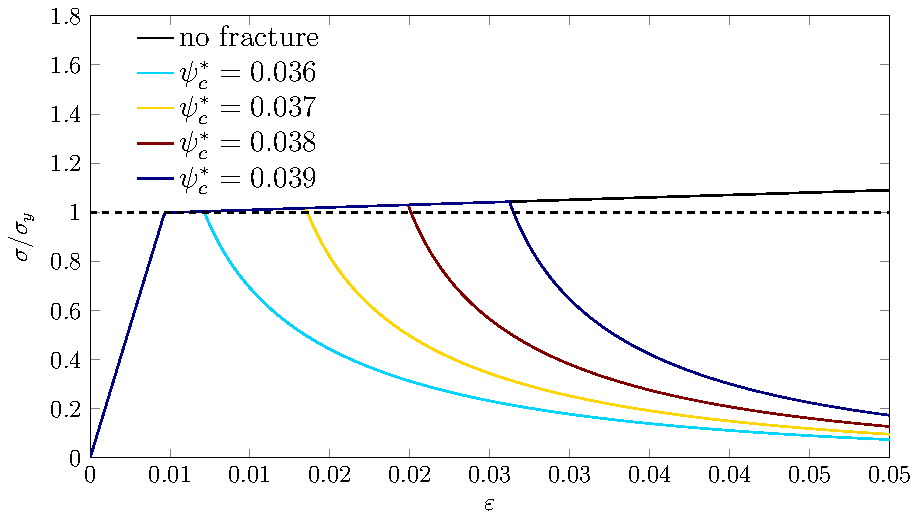
\includegraphics[width=0.9\textwidth]{theory/figures/Chapter5-homogenized-compare_alpha-EPD_xi_1}
              \end{figure}
            \end{column}
            \begin{column}[t]{0.5\textwidth}
              Issue: The response is regularization-length dependent.
              \begin{figure}
                \centering
                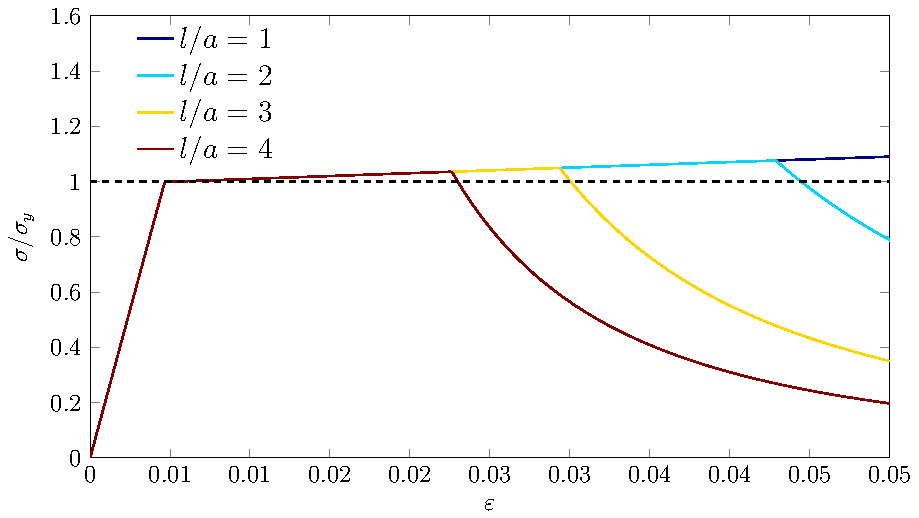
\includegraphics[width=0.9\textwidth]{theory/figures/Chapter5-homogenized-compare_degradation-EPPD_quad}
              \end{figure}
            \end{column}
          \end{columns}
        \end{column}
      \end{columns}
    }
    
    \only<4>{
      \begin{columns}
        \begin{column}{0.4\textwidth}
          \textboxed{Version 3} \\\bigskip
          
          Constitutive choices:
          \begin{align*}
            \psi^p     & = g \left( \sigma_y \ep + \dfrac{1}{2} H \ep^2 \right),     \\
            {\psi^p}^* & = 0,                                                        \\
            {\psi^f}^* & = \dfrac{1}{2} v \dot{d}^2,                                 \\
            \alpha     & = d,                                                        \\
            g          & = \textcolor{red}{\dfrac{(1-d)^2}{(1-d)^2 + m d (1-0.5d)}}. 
          \end{align*}
        \end{column}
        \begin{column}{0.6\textwidth}
          Resulting envelopes:
          \begin{align*}
            \norm{\dev(\bfM)} - \sqrt{\dfrac{2}{3}} \textcolor{red}{ \psi^p_{,\ep}}                                                                               & \leqslant 0,         \\
            \divergence \dfrac{2\Gc l}{c_0} \grad d - \left( \dfrac{\Gc}{c_0 l} \alpha_{,d} + \textcolor{red}{\psi^e_{,d}} + \textcolor{red}{\psi^p_{,d}} \right) & \leqslant v \dot{d}. 
          \end{align*}
          \begin{columns}
            \begin{column}[t]{0.5\textwidth}
              Improvement: The response is regularization-length dependent.
              \begin{figure}
                \centering
                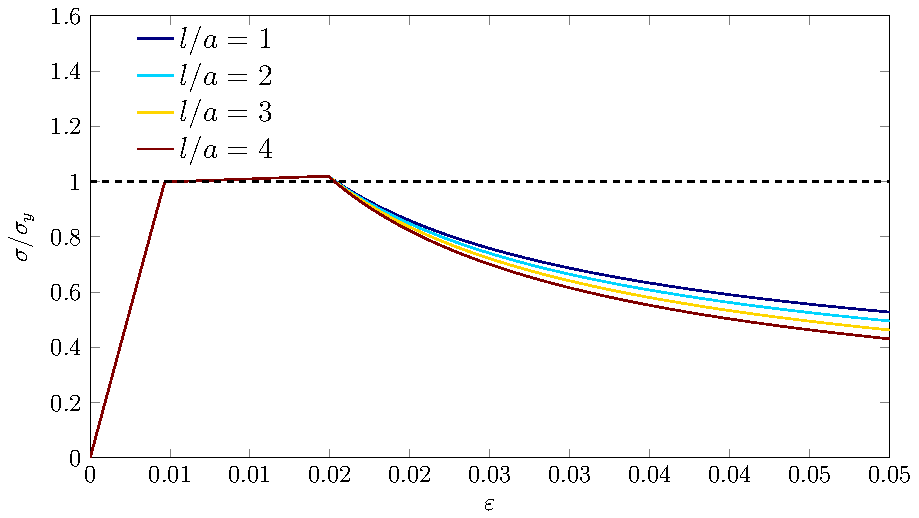
\includegraphics[width=0.9\textwidth]{theory/figures/Chapter5-homogenized-compare_degradation-EPPD_lorentz}
              \end{figure}
            \end{column}
            \begin{column}[t]{0.5\textwidth}
              Next: What if we incorporate thermal effects?
            \end{column}
          \end{columns}
        \end{column}
      \end{columns}
    }
    
    \only<5>{
      \begin{columns}
        \begin{column}{0.4\textwidth}
          \textboxed{Version 4} \\\bigskip
          
          Constitutive choices:
          \begin{align*}
            \textcolor{red}{\psi^p}     & \textcolor{red}{= (1-\tqf) g \sigma_y^T \ep, \quad {\psi^p}^* = \tqf g \sigma_y^T \epdot,} \\
            \textcolor{red}{\sigma_y^T} & \textcolor{red}{= \sigma_0 \exp\left( \dfrac{Q}{RT} \right),}                              \\
            {\psi^f}^*                  & = \dfrac{1}{2} v \dot{d}^2,                                                                \\
            \alpha                      & = d,                                                                                       \\
            g                           & = \dfrac{(1-d)^2}{(1-d)^2 + m d (1-0.5d)}.                                                 
          \end{align*}
        \end{column}
        \begin{column}{0.6\textwidth}
          Resulting envelopes:
          \begin{align*}
            \norm{\dev(\bfM)} - \sqrt{\dfrac{2}{3}} \left( \psi^p_{,\ep} \textcolor{red}{ + {\psi^p}^*_{,\epdot}} \right)                        & \leqslant 0,         \\
            \divergence \dfrac{2\Gc l}{c_0} \grad d - \left( \dfrac{\Gc}{c_0 l} \alpha_{,d} + \psi^e_{,d} + \textcolor{red}{\psi^p_{,d}} \right) & \leqslant v \dot{d}. 
          \end{align*}
          The variational framework also accounts for heat generation due to dissipative mechanisms:
          \begin{align*}
            \rho_0c_v\dot{T} & = \rho_0 q + \divergence \kappa \grad T + \textcolor{red}{\delta} + \textcolor{red}{\delta_T}, \\
            \delta           & = \bfP^\text{vis}:\dot{\defgrad} + {\psi^p}^*_{,\epdot}\epdot + {\psi^f}^*_{,\dot{d}}\dot{d},  \\
            \delta_T         & = {\psi^p}^*_{,\epdot T}\epdot T.                                                              
          \end{align*}
          Issue: To get a temperature increase, we need $\textcolor{red}{\tqf \geqslant \dfrac{Q}{Q+RT}}$.
        \end{column}
      \end{columns}
    }
    
    \only<6>{
      \begin{columns}
        \begin{column}{0.4\textwidth}
          \textboxed{Version 5} \\\bigskip
          
          Constitutive choices:
          \begin{align*}
            \psi^p     =                  & \  0, \quad {\psi^p}^* = g \sigma_y^T \epdot,                                                                             \\
            \sigma_y^T =                  & \ \sigma_0 \exp\left( \dfrac{Q}{RT} \right),                                                                              \\
            {\psi^f}^* =                  & \ \dfrac{1}{2} v \dot{d}^2 + \dfrac{\Gc}{c_0 l} \textcolor{red}{(1-C)} \dot{d}                                            \\
                                          & \ \textcolor{red}{- \dfrac{\Gc}{c_0l} (1-\beta) \left[ 1-\exp\left( -\dfrac{\ep}{\varepsilon_0} \right) \right]\dot{d}} , \\
            \alpha                      = & \ \textcolor{red}{C} d.                                                                                                   
          \end{align*}
        \end{column}
        \begin{column}{0.6\textwidth}
          Resulting envelopes:
          \begin{align*}
            \norm{\dev(\bfM)} - \sqrt{\dfrac{2}{3}} {\psi^p}^*_{,\epdot}                                                                       & \leqslant 0,         \\
            \divergence \dfrac{2\Gc l}{c_0} \grad d - \left( \dfrac{\textcolor{red}{\widehat{\Gc}}}{c_0 l} + \psi^e_{,d} + \psi^p_{,d} \right) & \leqslant v \dot{d}. 
          \end{align*}
          The fracture toughness is ``degraded'' by plastic deformation:
          \begin{align*}
            \widehat{\Gc} & = g^c \Gc, \quad g^c = 1-(1-\textcolor{red}{\beta})\left[ 1-\exp\left( -\dfrac{\ep}{\textcolor{red}{\varepsilon_0}} \right) \right]. 
          \end{align*}
          To satisfy the second law, part of the fracture process is made dissipative with the constraint:
          \begin{align*}
            0 < \textcolor{red}{C \leqslant \beta}.
          \end{align*}
        \end{column}
      \end{columns}
    }
  \end{overlayarea}
\end{frame}
